\subsection{EXTENSION OF THE RING OF SCALARS}

Let A, A' be two commutative rings, \(\rho:A\to A'\) a ring homomorphism, M an A-module, M' an A'-module and \(f:M\to M'\) an A-homomorphism (relative to \(\rho\) ) of M into M'. The composite mapping \(M\xrightarrow{f}M'\xrightarrow{\phi_{M'}^{\prime\prime}}\bigwedge_{A'(M')}\) is an A-linear mapping of M into the A-algebra \(\bigwedge_{A'(M')}\) and, as the elements of \(f(\mathbf{M}) \subset \mathbf{M}'\) are of zero square in \(\bigwedge_{\mathbf{A}'}(\mathbf{M}')\) , there exists (no. 1, Proposition 1) one and only one A-homomorphism of algebras \(f'': \bigwedge_{\mathbf{A}}(\mathbf{M}) \to \bigwedge_{\mathbf{A}'}(\mathbf{M}')\) rendering commutative the diagram

\begin{enumerate}
\def\labelenumi{(\arabic{enumi})}
\setcounter{enumi}{11}
\tightlist
\item
\end{enumerate}

\pandocbounded{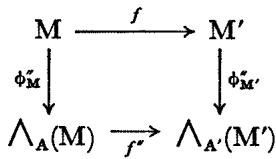
\includegraphics[keepaspectratio]{images/part003_899f4c21.jpg}}

and \(f''\) is a graded algebra homomorphism. It is immediately deduced that if \(\sigma: A' \to A''\) is another ring homomorphism, \(M''\) an \(A''\) -module, \(g: M' \to M''\) an \(A'\) -homomorphism (relative to \(\sigma\) ) and \(g'': \bigwedge_{A'}(M') \to \bigwedge_{A''}(M'')\) the corresponding \(A''\) -homomorphism of algebras, then the composite A-homomorphism of algebras

\[
\bigwedge_ {\mathbf {A}} (\mathbf {M}) \xrightarrow {f ^ {\prime \prime}} \bigwedge_ {\mathbf {A} ^ {\prime}} (\mathbf {M} ^ {\prime}) \xrightarrow {g ^ {\prime \prime}} \bigwedge_ {\mathbf {A} ^ {\prime \prime}} (\mathbf {M} ^ {\prime \prime})\tag{13}
\]

corresponds to the composite A-homomorphism \(g \circ f: \mathbf{M} \to \mathbf{M}''\) (relative to \(\sigma \circ \rho\) ).

PROPOSITION 8. Let A, B be two commutative rings, \(\rho: A \to B\) a ring homomorphism and M an A-module. The canonical extension

\[
\psi : \bigwedge_ {\mathbf {B}} (\mathbf {B} \otimes_ {\mathbf {A}} \mathbf {M}) \rightarrow \mathbf {B} \otimes_ {\mathbf {A}} \bigwedge_ {\mathbf {A}} (\mathbf {M})
\]

of the B-linear mapping \(l_{B} \otimes \phi_{M}^{\prime\prime}: B \otimes_{A} M \to B \otimes_{A} \bigwedge_{A}(M)\) is a graded B-algebra isomorphism.

The proof is derived from that of § 5, no. 4, Proposition 5 replacing T by \(\bigwedge\) and \(\phi_{\mathbf{M}}\) by \(\phi_{\mathbf{M}}^{\prime \prime}\) .

